\documentclass[12pt]{article}
\input{knitr.tex}
\usepackage{graphicx}
\usepackage{placeins}
\usepackage{float}
\usepackage{grffile}
\usepackage{color}
\usepackage{soul}
\usepackage{tabularx}
\usepackage{multirow}
% use \xspace to allow for space after a macro as necessary
\usepackage{xspace}
\usepackage{pdfpages}
\usepackage[top=1in, bottom=1in, left=1.25in, right=1.25in]{geometry}

\definecolor{commentcol}{rgb}{0.345, 0.345, 0.945}
\newcommand{\comment}[1]{\textcolor{commentcol}{[[#1]]}}%
\newcommand{\code}[1]{\texttt{#1}}

% general-purpose mathrm macros
\newcommand{\symsub}[2]{\ensuremath{#1_{\tiny \mathrm{#2}}}\xspace}
\newcommand{\mrm}[1]{\ensuremath{\mathrm{#1}}
\xspace}

\usepackage{framed}

\definecolor{randomcolor}{rgb}{.97, .27, .67}
\definecolor{shadecolor}{rgb}{.97, .97, .97}
\definecolor{messagecolor}{rgb}{0, 0, 0}
\definecolor{warningcolor}{rgb}{1, 0, 1}
\definecolor{errorcolor}{rgb}{1, 0, 0}

\usepackage{alltt}
\usepackage[]{natbib}
\usepackage{blkarray}
\usepackage{amsmath}
\usepackage{alltt}
\usepackage{hyperref}
\usepackage[utf8]{inputenc} % for accented characters

%% \pagenumbering{gobble}
%% stuff for editing
%\usepackage[markup=nocolor,addedmarkup=bf,deletedmarkup=sout]{changes}
%% to suppress notes & comments: \usepackage[final]{changes}
\usepackage{setspace}
%% \usepackage{changes} %%% Not playing well with others!
%% \usepackage[backgroundcolor=lightgray,textsize=tiny]{todonotes}
\usepackage[]{todonotes}

\bibliographystyle{chicago}
\title{Reassessing global historical \rzero estimates of canine rabies}
\author{Michael Li, Michael Roswell, Katie Hampson, Ben Bolker and Jonathan Dushoff}

\providecommand{\keywords}[1]{\textbf{\textit{Keywords:}} #1}
\IfFileExists{upquote.sty}{\usepackage{upquote}}{}
\begin{document}
%% \SweaveOpts{concordance=TRUE}
\newcommand{\dbic}{\ensuremath \Delta \texttt{BIC}}

\newcommand{\bmb}[1]{\comment{BB: #1}}
\newcommand{\jd}[1]{\comment{JD: #1}}
\newcommand{\kh}[1]{\comment{KH: #1}}
\newcommand{\mli}[1]{{\color{red} ML: #1}}
\newcommand{\mr}[1]{{\color{blue} MR: #1}}

\newcommand{\eqnref}[1]{Eq~\eqref{eq:#1}}
\newcommand{\eqnlabel}[1]{\label{eq:#1}}

\newcommand{\fref}[1]{Figure~\ref{fig:#1}}
\newcommand{\Fref}[1]{Figure~\ref{fig:#1}}
\newcommand{\flabel}[1]{\label{fig:#1}}

\newcommand{\add}[1]{{\color{blue} ADD: #1}}

\newcommand{\rzero}{\ensuremath{{\mathcal R}_0}\xspace}
\newcommand{\re}{\ensuremath{{\mathcal R}_{e}}\xspace}

\newcommand{\littler}{\ensuremath{r_0}\xspace}

\newcommand{\Gx}{\textsl{G}}
\newcommand{\G}{\Gx\xspace}
\newcommand{\Gs}{\Gx \xspace}

\newcommand{\SIx}{\textsl{SI}}
\newcommand{\SI}{\SIx\xspace}
\newcommand{\SIs}{\SIx s\xspace}

%% END MACROS SECTION

%\SweaveOpts{concordance=TRUE}
%\SweaveOpts{concordance=TRUE}
% \maketitle

{\Large
\textbf\newline{Reassessing global historical \rzero estimates of canine rabies} % Please use "sentence case" for title and headings (capitalize only the first word in a title (or heading), the first word in a subtitle (or subheading), and any proper nouns).
}
\newline
% Insert author names, affiliations and corresponding author email (do not include titles, positions, or degrees).
\\
Michael Li\textsuperscript{1,2*},
Michael Roswell \textsuperscript{1,3},
Katie Hampson\textsuperscript{4},
Benjamin M. Bolker\textsuperscript{1,2,5},
Jonathan Dushoff\textsuperscript{1,2,5}
\\
\\
\\
* Corresponding author: lim88@mcmaster.ca \\
\textbf{1} Department of Biology, McMaster University, Hamilton, Ontario, Canada
\\
\textbf{2} Department of Mathematics and Statistics, McMaster University, Hamilton, Ontario, Canada
\\
\textbf{3} Department of Biology, University of Maryland, College Park, Maryland,  USA
\\
\textbf{4} Institute of BAH\&CM, University of Glasgow, Glasgow, UK
\\
\textbf{5} Institute for Infectious Diseases Research, McMaster University, Hamilton, Ontario, Canada
\\
\bigskip

% Insert additional author notes using the symbols described below. Insert symbol callouts after author names as necessary.
%
% Remove or comment out the author notes below if they aren't used.
\doublespacing

\keywords{incubation period, infectious period, generation interval}


\section*{Abstract}

% Please keep the Author Summary between 150 and 200 words
%% current length not including comments: 197 words
Rabies spread by domestic dogs continues to cause tens of thousands of human deaths every year in low- and middle-income countries. Nevertheless rabies is often neglected, perhaps because it has already been eliminated from high-income countries through dog vaccination.
%% \mr{Maybe discuss neglect elsewhere; there are issues.} \mli{Rephrased a bit, not seeing a big issue in general.}
Estimates of canine rabies's intrinsic reproductive number (\rzero), a metric of disease spread, from a wide range of times and locations are relatively low (values $<2$), with narrow confidence intervals. Given rabies's persistence, this consistently low and narrow range of estimates is surprising.
We combined incidence data from historical outbreaks of canine rabies from around the world with in-depth contact-tracing data from Tanzania to investigate initial growth rates (\littler), generation-interval distributions (\G), and reproductive numbers (\rzero).
We improved on earlier estimates by choosing outbreak windows algorithmically; fitting \littler using a more appropriate statistical method that accounts for decreases through time; and incorporating uncertainty from both \littler and \G in our confidence intervals on \rzero. 
Our \rzero estimates are larger than previous estimates, with wider confidence intervals.
Our novel hybrid approach for estimating \rzero and its uncertainty is applicable to other disease systems where researchers estimate \rzero by combining data on \littler and \G.
%\mr{is it still a "hybrid" approach now that uncertainty is estimated via bootstraps rather than a Bayesian  MCMC sampler?} 

% \linenumbers %% switch for line number

\section*{Introduction}

Canine rabies, primarily spread by domestic dogs, is a vaccine-preventable disease that continues to cause tens of thousands of human deaths every year in low- and middle-income countries (LMICs)
\citep{taylor2017difficulties, minghui2018new}.
Canine rabies has been effectively eliminated from high-income countries by mass dog vaccination \citep{rupprecht2008can}.
Despite the effectiveness of dog vaccination, rabies continues to cause many human deaths and large economic losses in LMICs due to the limited implementation of rabies control strategies \citep{hampson2015estimating}. 
The past two decades have seen an increase in rabies control efforts, including dog vaccination campaigns and improvements in surveillance \citep{kwoba2019dog, mtema2016mobile, gibson2018one, mazeri2018barriers, wallace2015establishment}.
The World Health Organization (WHO) and partners (OIE, FAO, GARC) joined forces to support LMICs in eliminating human deaths from dog-mediated rabies by 2030 \citep{minghui2018new, abela20162016}. Mass dog vaccination campaigns have begun in some LMICs and are being scaled up \citep{castillo2019socio, evans2019implementation}.
However, the emergence of SARS-CoV-2 pandemic disrupted rabies control and elimination efforts \citep{nadal2022impact}.
As the SARS-CoV-2 pandemic is transitioning out of global emergency, rabies control programmes are resuming.
% https://www.who.int/news-room/fact-sheets/detail/rabies
An understanding of rabies epidemiology --- in particular, reliable estimates of the basic reproductive number (\rzero), a quantitative measure of disease spread that is often used to guide vaccination strategies --- could inform rabies control efforts.

The basic reproductive number \rzero is defined as the expected number of secondary cases generated from each primary case in a fully susceptible population \citep{macdonald1952analysis}.
% KH edited below to split lengthy sentence
Estimates of \rzero for rabies have been made using various methods including direct estimates from infection histories, epidemic tree reconstruction, and epidemic curve methods. These \rzero estimates based on historical outbreaks of rabies have generally been surprisingly low, typically between 1 and 2 with narrow confidence intervals for a variety of regions and time periods \citep{hampson2009transmission, kurosawa2017rise, kitala2002comparison}. 
With such a low \rzero one might expect rabies to fade out due to a combination of behavioural control measures and stochastic fluctuations, even in the absence of vaccination.
In contrast to diseases with a large \rzero (e.g., rinderpest, with \rzero $\approx 4$ \citep{mariner2005model}), \rzero estimates for rabies suggest that control through vaccination should be relatively easy.

% \rzero estimates for rabies using various methods (i.e., direct estimates from infection histories, epidemic tree reconstruction and have been consistently low, with narrow confidence intervals \citep{hampson2009transmission}.
Here we revisit and explore why rabies, with its low \rzero, nonetheless persists in many countries around the world. 
Such persistence suggests that rabies's potential for spread, and therefore the difficulty of rabies control, may have been underestimated. 
In this paper, we combine information derived from epidemic curves with a high-resolution contact tracing data set that provides large numbers of observed generation intervals (which is rare for infectious disease studies) to estimate \rzero.
%% This reassessment can reevaluate the estimation of $\rzero$ for rabies outbreaks and understanding of disease control more generally.
%% \mr{I think the "more generally" part desserves a bit more preamble/evidence... maybe this is a bit late to get to the general overall, although this may depend where you're publishing and the hopes that this can spur rabies vaccination campaigns} \mli{Happy to get rid of it.}
%% need a \rzero P about euler and bad CI

\section*{Materials and Methods}

\rzero is often estimated by combining two other epidemiological quantities: the initial growth rate of an epidemic (\littler) and the generation interval (\G) distribution, where the generation interval is defined as the time between successive infections along a transmission chain \citep{park2018exploring}.
The initial growth rate \littler is often estimated by fitting a model to time series data from the early stages of epidemics.
\G is an individual-level quantity that measures the time between an individual getting infected to infecting another individual.
The generation interval distribution is the natural way to link \littler and \rzero \citep{wallinga2006generation, champredon2015intrinsic}.
\rzero can be estimated from \littler and the \G distribution
by the Euler-Lotka equation \citep{wallinga2006generation}
\begin{equation}
\rzero = \frac{1}{\sum_{t=1}^{\infty} G(t)e^{-rt}},
\label{eq:EL}
\end{equation}
where $t$ is time, and $G(t)$ is the generation interval distribution.
This formula is convenient to calculate point estimates of \rzero; however, researchers rarely propagate uncertainty from the estimates of \littler and the \G distribution through this formula.

\subsection*{Initial growth rate}

Disease incidence typically increases approximately exponentially during the early stages of an epidemic. The initial growth rate \littler is often estimated by fitting exponential curves from near the beginning to near the peak of an epidemic.
However, growth rates estimated from an exponential model can be biased downward, overconfident, and sensitive to the choice of fitting windows \citep{ma2014estimating}.
Here we used logistic rather than exponential curves to more robustly estimate \littler \citep{ma2014estimating, chowell2017fitting}.
%% \mr{This seems like such a big piece of the difference between KH and WZLi estimates; I'm surprised it only gets mentioned here in M\&M but not highlighted in abstract/methods. Especially since KH is an author, seems fine to be more firm in claiming logistic is more appropriate and likely to resolve some of the "paradox"\\ } \mli{Added a few words in the abstract.}

%\mr{code-formatted variable names may be alienating, maybe describe in more conventional terms with either just words, or mathy variable names?}
We selected fitting windows algorithmically for each outbreak as follows: (1) we break each time series into “phases”: a new phase starts after a peak with a height of at least \code{minPeak} cases, followed by a proportional decline in cases of at least \code{declineRatio}; (2) In each phase, we identify a prospective fitting window starting after the last observation of 0 cases and extending one observation past the highest value in the phase (unless the highest value is itself the last observation); (3) we then fit our model to the cases in the fitting window if (and only if) it has a peak of at least \code{minPeak} cases, a length of at least \code{minLength} observations, and a ratio of at least \code{minClimb} between the highest and lowest observations. We tried a handful of parameter combinations before settling on a final set during an expert consultation. These explorations are detailed, and the final choices noted, in our code repository.
%% \kh{Can we report these values - minPeak, declineRatio, minClimb and minLenght here too, while also referring readers to the repo notes?} 

\subsection*{Observed Generation intervals}

Transmission events are hard to observe directly for most diseases. %% \kh{ revised to get rid of influential - feels awkward to read as one of the current authors! }
An earlier empirial rabies study constructed generation intervals by summing two quantities: a latent period (the time from infection to infectiousness), and a wait time (time from infectiousness to transmission) \citep{hampson2009transmission}.
Since clinical signs and infectiousness appear at nearly the same time in rabies, the incubation period (the time from infection to clinical signs) is routinely used as a proxy for the latent period.
\citeauthor{hampson2009transmission} randomly and independently resampled latent (really, incubation) periods and infectious periods from empirically observed distributions \citep{hampson2009transmission}, and then sampled waiting times uniformly from the selected infection periods.

However, constructing \G values by summing independently resampled values of incubation and infectious periods accounts neither for the possibility of multiple transmissions from the same individual, nor for correlations between time distributions and biting behaviour.
\fref{intervals} illustrates the generation intervals of a single transmission event from a rabid animal (comprising a single incubation period plus a waiting time) and multiple transmission events from a rabid animal (comprising a single incubation period and three waiting times).
%% \kh{Serial-interval terminology used below (only time in ms). But I think this is somewhat confusing. It might need more introduction?}
In cases where transmission links are not directly observed, one should consider reweighting serial-interval observations to account for  multiple transmissions. In our case, we can account for these effects directly by relying on generation intervals observed through contact tracing.

\begin{center}
\begin{figure}[ht!]
\includegraphics[scale = 0.5]{./interval.png}
\caption{\textbf{Decomposing generation intervals.}
Generation intervals start when a focal animal acquires infection (open red circle) and end after a period of viral replication (dashed line) when an animal shows clinical signs (blue star), becomes infectious (solid black circle) and infects another animal --- in rabies, the onset of clinical signs and of infectiousness are closely synchronized.
Once the infectious period (grey block) starts, there is a wait time (solid black line) until a susceptible host (solid red circles) is bitten. The infectious period ends with the death of the focal host (black X).
The generation interval is the interval between the focal animal getting infected, and when it infects a new case (red interval between open and solid circles). If a single biter transmits multiple times (right), the wait times generally vary, but the incubation period is the same for each transmission event.}
\flabel{intervals}
\end{figure}
\end{center}

\FloatBarrier

\subsection*{Correcting for vaccination}

In a population where some animals are not susceptible, calculations based on estimates of \littler and the \G distribution (\ref{eq:EL}) estimate the \emph{realized} average number of cases per case, also known as the effective reproductive number \re.
In the case of rabies, vaccination is the only known cause of immunity (case fatality in dogs is believed to be 100\%).
For a given population with $\nu$ vaccination proportion, the estimated $\rzero$ with correction for vaccination is
\begin{equation}
\rzero = \frac{\re}{(1 - \nu)}.
\label{eq:RE}
\end{equation}

\subsection*{Data}



We used data from December 2002 -- November 2022, from an ongoing contact tracing study in Tanzania \citep{hampson2008rabies, hampson2009transmission}.
The data set contains 8636 domestic dog recorded events (i.e., domestic dogs bitten by an animal), and 3552 suspected rabid dogs in the Serengeti District of northern Tanzania.
Transmission events were documented through retrospective interviews with witnesses, applying diagnostic epidemiological and clinical criteria from the six-step method \citep{tepsumethanon2005six}.
Each dog was given a unique identifier, and date of the bite and clinical signs were recorded if applicable and available.
2132 of the dog transmissions were from unidentified domestic animals or wildlife.
We restricted our analysis to domestic dog transmissions (i.e., dog to dog), and obtained 293 directly observed generation intervals (i.e. both biter and secondary case have ``time bitten" records).
There were four observed dogs with multiple exposures (i.e., bitten by different identified biters), generating extra generation intervals, but it is unclear which transmission event transmitted rabies to these dogs.
For simplicity, we omitted these four dogs and their generation intervals from our analysis.

\subsection*{Fitting and Propagating Parameter Uncertainties}



To propagate uncertainties for both \littler and \G, we used a hybrid approach.
We first fit logistic models, with negative binomial observation error, to incidence data to estimate \littler implemented in the R package {\tt epigrowthfit} \cite{epigrowthfit}.
We then compute a sample of 1000 $\hat{\rzero}$ values using equation (\ref{eq:RE}).
For each value of $\hat{\rzero}$, we first draw a value of $\hat{\littler}$ from a Normal distribution matching the estimated sampling distribution of the logistic fit parameters and an independent sample of \G from the empirical contact tracing data. To sample \G from the empirical contact tracing data, we first take a weighted sample of 100 biters, which accounts for biter-level variation, and for each biter, we sample a \G from its respective transmission event, to account for individual variation.
We then matched samples of \G to the \littler samples to produce a range of estimates for \rzero.
This hybrid sampling approach incorporates the uncertainties in both \littler and \G
into the distribution of \rzero estimates.
Finally, we use the 2.5, 50,  and 97.5 percentiles of the distribution of \rzero estimates to get point estimates and confidence limits for $\rzero$ for each rabies outbreak.

\section*{Results}

\begin{center}
\begin{figure}[ht!]
\includegraphics[page=1,scale=0.7]{intervalPlots.Rout.pdf}
\caption{\textbf{Time intervals and biting empirical distributions from contact tracing data.}
%\mr{replace caption with a description of the takehome point of the figure?}
Panel A is the distribution of observed incubation periods. Panel B is the distribution of incubation periods weighted by each dog's biting frequency (Panel C). The weighted distribution corresponds to the contribution of incubation periods to generation intervals (Panel D).
Black dashed lines show the means of each time-interval distribution; blue dashed lines show the mean incubation period and generation interval (22.3 and 24.9 days, respectively) reported by \cite{hampson2009transmission}.
}
\flabel{GISI}
\end{figure}
\end{center}

\FloatBarrier

\Fref{GISI} shows the empirical distributions of the observed incubation periods, rabid dog biting frequency, and generation intervals from contact tracing data.
The mean observed incubation period is 27.5 days ($n = 1109$ dogs), the mean biting frequency is 1.65 bites per rabid dog, and the weighted mean incubation period is 36.6 days ($n = 143$ biting dogs).
The mean observed generation interval is 37.9 days ($n = 143$ primary infections resulting in 293 secondary cases), which is substantially larger than the mean generation interval constructed from summing independently sampled incubation periods and wait times (24.9 days \citep{hampson2009transmission}).
The weighted incubation period distribution is a better approximation of the generation interval distribution than the unweighted incubation period of all dogs.

\begin{center}
\begin{figure}[h]
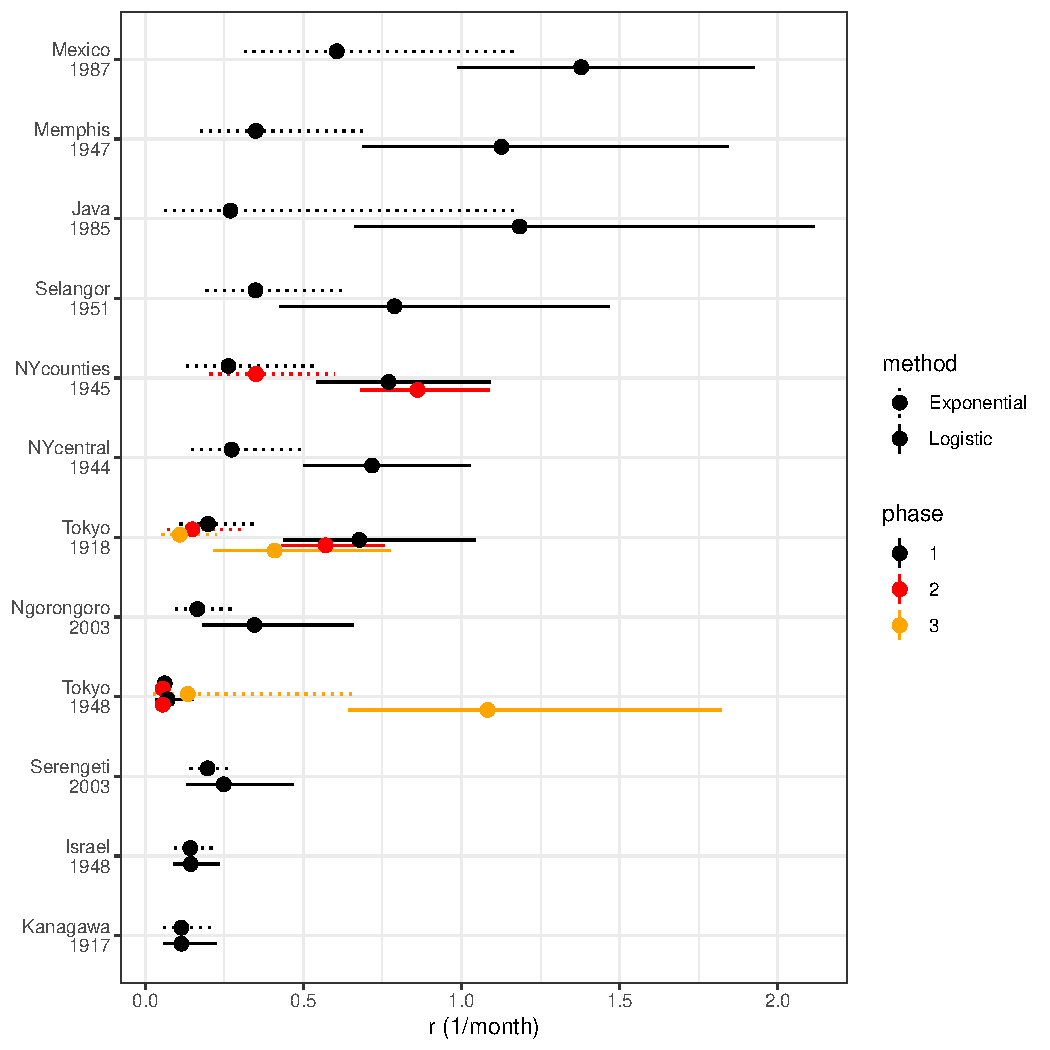
\includegraphics[page=1,scale = 0.7]{rplot_combo.Rout.pdf}
\caption{\textbf{Growth rate estimates for global historical outbreaks of rabies.} Estimates and 95\% confidence intervals of \littler in global historical outbreaks estimated from exponential (dotted) and logistic (solid) model fits.}
Different colors represent different phases from the times series data.
\bmb{this could be prettier (non-default colours, shapes as well as colours to identify phases,
  maybe use solid lines for logistic since we want to emphasize it, rotate lines in legend to be
  horizontal ...) ?}
\mli{Rotating the lines in legend seems hard. Have to use geom segment and it doesn't play well with position dodge. %https://stackoverflow.com/questions/58761704/dodged-dumbbell-plots-with-ggplot2
}  
\flabel{littler}
\end{figure}
\end{center}

\FloatBarrier

We estimated \littler from historical outbreak data (\fref{littler}). 
For a direct comparison of the method used in \citep{hampson2009transmission}, we also estimated \littler from an exponential model. Both methods (exponential and logistic) were applied to all phases of the global historical outbreaks. 
Overall, \littler estimates from the logistical model are larger with wider confidence intervals compared to \littler estimates from the exponential model (as used in \citep{hampson2009transmission}). 

\begin{center}
\begin{figure}[h]
\includegraphics[page=1,scale = 0.7]{R0combo.Rout.pdf}
\caption{\textbf{Reproductive number estimates for global historical outbreaks of rabies}}
Previous estimates of \rzero are shown in blue highlights; \rzero estimates and confidence interval (95\% quantiles from the estimated \rzero sample) from our hybrid approach using exponential (dotted lines) and logistic (solid lines). \rzero values are corrected for vaccination coverage.
\bmb{What did the previous esimates do about phases?}
\mli{The previous estimates did not have phases.}
\flabel{Rzero}
\end{figure}
\end{center}

\FloatBarrier

We combined our estimates of \littler from the logistic model with the empirical \G from our detailed Tanzanian data to produce \rzero estimates.
Of the listed historical outbreaks, four occurred in locations with prior rabies vaccination coverage: Memphis and Shelby County, Tennessee, US (``Memphis'': 1947, 10\% vaccine coverage); Serengeti, Tanzania (2003, 20\% coverage); Ngorongoro, Tanzania (2003, 20\% coverage); and Sultan Hamad, Kenya (1992, 24\% coverage).
\fref{Rzero} shows the \rzero estimates using various approaches along with estimates from \cite{hampson2009transmission}. 
Our estimates of \rzero using the logistic model and corrected \G are larger than those previously reported \citep{hampson2009transmission}, with 3 locations (Java, Memphis, and Mexico) having \rzero greater than 2.
The hybrid approach provides larger values of \rzero and wider confidence intervals after propagating uncertainty from both \littler and generation interval distributions with upper confidence limits greater than 2 for most locations.

% \mr{you set up the idea that R0 should vary across populations, but I don't think very clearly yet (density seems like a good one, since the idea behind R0 is that it includes both the contact rate and the transmission rate). But you use a single region to estimate generation intervals... can you state a bit about why this seems like a fine assumption (i.e., something like you expect similar variation in dogs within and across populations -- even though the other paper is all about how important the dog-to-dog variation in latent period is for understanding dynamics?) Is this line of thinking citeable?}
% \mli{Maybe put this in the discussion or methods?} 

\FloatBarrier

\begin{center}
\begin{figure}[h]
\includegraphics[page=1,scale = 0.7]{mexico.Rout.pdf}
\caption{\textbf{Effects of \littler estimation methods and corrected \G on the estimates of \rzero in Mexico outbreak.}
``Exponential'' represents a fitting method similar to that used by \cite{hampson2009transmission}, but using our algorithmic windowing selection; ``Logistic'' uses a logistic model instead. ``Naive GI'' uses the \G estimates from \cite{hampson2009transmission}; ``Corrected GI'' uses the resampling method described above. Both switching from exponential to logistic fitting, and using the corrected \G estimate, lead to increases in the estimated $\rzero$.  Propagating the uncertainty of \littler and \G estimates increases uncertainty in $\rzero$.
%\bmb{Make this horizontal to match the other figs? Extend R0-axis to have a lower limit at \rzero=1? Make $\rzero$ prettier (e.g. using tikzDevice)?}
%\mr{what ben said :-)}
%\mli{I actually like it this way.}
%\bmb{why?}
%\mli{to show this is a different type of plot}
}
\flabel{mexico}
\end{figure}
\end{center}

\FloatBarrier

Lastly, we compare the effects of different estimation techniques of \littler and \G on estimates of \rzero (\fref{mexico}). 
For illustrative purposes, we used the 1987 outbreak in Mexico where there was no vaccination. 
Propagating uncertainty from both \littler and \G generally leads to wider confidence intervals compared to previous \rzero estimates in \citet{hampson2009transmission}.
The \rzero estimate increases when we estimate \littler via the logistic model, or when we sample the full distribution of \G, rather than plugging in the naively constructed interval as in \cite{hampson2009transmission} .
Combining the two corrections (in \littler and \G) boosts the \rzero estimates even more, with even wider confidence intervals.

\section*{Discussion}

Our study resolves the mystery of why rabies persists despite the fact that \rzero estimates in historical outbreaks have been consistently low, by showing that substantially higher basic reproduction numbers are compatible with historical outbreak data.
Here, we reanalyzed historical rabies epidemics with improved model assumptions and uncertainty propagation, showing that historical estimates of \rzero were downward biased and overconfident.

The basic reproductive number, \rzero, is commonly used to summarize the risk of infectious disease and to inform control measures. Here, we used a relatively simple approach to estimating \rzero by combining initial growth rate (\littler) estimates from incidence data and generation intervals from contact tracing data.
By assuming rabies generation intervals are similar across time and space, this method allows us to combine generation intervals from the detailed Tanzania contact tracing data with growth rates estimated from incidence data from various regions across the globe. 
We improved on earlier work by correcting for slowdown in epidemic growth when estimating \littler, and by developing an approach to propagate uncertainty from both \littler and \G, resulting in higher \rzero estimates with wider confidence intervals.

Estimates of \rzero are strongly affected by estimates of the growth rate during the initial phase of the epidemic.
The logistic model gives a better approximation of the initial phase of the epidemic resulting in a larger estimate of \littler compared to the exponential model \citep{ma2014estimating}.
Our estimates of \littler account for observation error (measurements may not perfectly match reality), but not for process error (the fundamental stochasticity of the system itself). Thus we may still be underestimating the uncertainty in \littler, and hence in \rzero \citep{king2015avoidable}.
%\mr{is the point here to contrast with the way you used a more complete distribution of G to account for process error on that side of the equation?}

Re-analysis of these data also allowed us to identify an overlooked fact about rabies generation intervals: observed generation intervals are longer, on average, than intervals constructed by naively adding incubation period and waiting time, because of within-individual correlations in time distributions and biting behaviour. The unexpected importance of these correlations could have implications for other infectious disease analyses that depend on the generation interval, as such correlations can bias the estimation of generation intervals, as shown in this study. Further investigation of how these correlations affect the overall dynamics of rabies is warranted.

In any case, our estimates suggest that the \rzero of rabies is larger, and more uncertain, than previously estimated.
This finding may explain some of the formerly unexplained variations in the success of rabies-control programs (e.g., low levels of coverage (30–50\%) have succeeded in some settings while high coverage 75\% was insufficient to control rabies in others \citep{eng1993urban}).
While our primary goal was to understand why estimates of rabies \rzero were small with narrow confidence intervals, our analysis also revealed an interesting biological process through the lens of generation intervals from contact tracing data: the need to account for biting behaviour in the incubation period distribution, in order to match the generation interval distribution.
 
\rzero is typically used as a first approximation for interventions such as vaccination to determine herd immunity thresholds. 
However, both heterogeneity in contacts and the correlations between incubation periods and transmission that we observed here through the generation interval suggest that simple \rzero estimation methods should be used with caution. 
Rabies is particularly useful for exploring this effect because transmission events and latent periods are directly observable via contact tracing. The correlation effect highlighted here is likely to apply in other disease systems, but hard to detect because generation intervals are so rarely directly observable.

%\mr{not sure which paper is destined to come out first, or if you're subitting them (i.e., this one an correlations paper) together somehow... I think there could be a more explicit linking between the two papers. I think the sentence Ben suggested you refine could be more positive: you advocate estimating R0 with uncertainty propagation (and also why logistic is more appropriate than exponential, and how general you think that should be. I don't love landing on the mechanistic fitting suggestion; think it would be good to end on strong sentences focused on take-home messages.) Consider moving most of last paragraph up to first in discussion. I think more can be said about how Rabies is a nice model system because latent period and transmission events are so easy to observe, and natural immunity is not thought to exist, but your findings can be applicable in disease systems where the uncertainties in generation interval may be even greater, or something like that.}
%\mli{suggstion accepted}


\singlespacing

\bibliography{rabies}

\end{document}
